\documentclass[compress]{beamer}

\usetheme{m}

\title{Titel der supertollen Arbeit}
\subtitle{Untertitel}
\date{\today}
\author{Max Mustermann --- max.mustermann@foo.com}
\institute{Institut für so und so\\Universtität Bla}


\begin{document}

\maketitle


\section{Motivation}

\begin{frame}{Viel text}
Lorem ipsum dolor sit amet, consetetur sadipscing elitr, sed diam nonumy eirmod
tempor invidunt ut labore et dolore magna aliquyam erat, sed diam voluptua. At
vero eos et accusam et justo duo dolores et ea rebum. Stet clita kasd gubergren,
no sea takimata sanctus est Lorem ipsum dolor sit amet. Lorem ipsum dolor sit
amet, consetetur sadipscing elitr, sed diam nonumy eirmod tempor invidunt ut
labore et dolore magna aliquyam erat, sed diam voluptua. At vero eos et accusam
et justo duo dolores et ea rebum. Stet clita kasd gubergren, no sea takimata
sanctus est Lorem ipsum dolor sit amet.
\end{frame}


\section{Elements}

\begin{frame}{Lists}
  \begin{itemize}
    \item Hello
    \item Hello \emph{you}
    \item htt \url{http://google.com}
  \end{itemize}

  \begin{enumerate}
    \item \alert{important}
    \item Two
    \item Three
  \end{enumerate}
\end{frame}

\begin{frame}{Animation}
  \begin{itemize}[<+- | alert@+>]
    \item Hey
    \item \alert<4>{Ho}
    \item Let's go
  \end{itemize}
\end{frame}

\begin{frame}{Figures}
  \begin{figure}
    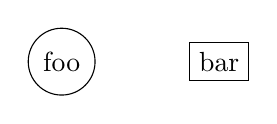
\begin{tikzpicture}
      \node[circle, draw=black] at (0, 0) {foo};
      \node[rectangle, draw=black] at (2, 0) {bar};
    \end{tikzpicture}
    \caption{Circle and rectangle}
  \end{figure}
\end{frame}

\begin{frame}{Blocks}
  \begin{block}{Fancy block title}
    Block inside
  \end{block}

  Outside
\end{frame}

\begin{frame}{Math}
  \begin{equation*}
    I_c(x,y) = \sum_{i=-n}^n\sum_{j=-n}^n w\left(
      \mathcal{N}_{x,y},\ \mathcal{N}_{x-i, y-j}\right)
      \cdot
      I_r(x-i,y-j)
  \end{equation*}
\end{frame}


\section{Conclusion}

\begin{frame}{Summary}
  Last words.
\end{frame}

\statement{Questions?}

\end{document}
